% -*- latex -*-
%%%%%%%%%%%%%%%%%%%%%%%%%%%%%%%%%%%%%%%%%%%%%%%%%%%%%%%%%%%%%%%%
%%%%%%%%%%%%%%%%%%%%%%%%%%%%%%%%%%%%%%%%%%%%%%%%%%%%%%%%%%%%%%%%
%%%%
%%%% This text file is part of the source of 
%%%% `Introduction to High-Performance Scientific Computing'
%%%% by Victor Eijkhout, copyright 2012/3/4/5/
%%%%
%%%% This book is distributed under a Creative Commons Attribution 3.0
%%%% Unported (CC BY 3.0) license and made possible by funding from
%%%% The Saylor Foundation \url{http://www.saylor.org}.
%%%%
%%%%
%%%%%%%%%%%%%%%%%%%%%%%%%%%%%%%%%%%%%%%%%%%%%%%%%%%%%%%%%%%%%%%%
%%%%%%%%%%%%%%%%%%%%%%%%%%%%%%%%%%%%%%%%%%%%%%%%%%%%%%%%%%%%%%%%

For operations to be executable in parallel they need to be independent.
That makes recurrences problematic to evaluate in parallel.
Recurrences occur in obvious places such as solving a triangular system 
of equations (section~\ref{sec:lu-solve}),
but they can also appear in sorting and many other operations.

In this appendix we look at \emph{parallel prefix} operations: the
parallel execution of an operation that is defined by a recurrence
involving an associative operator.  Computing the sum of an array of
elements is an example of this type of operation (disregarding the
\emph{non-associativy}\index{floating point
  arithmetic!associativity of} for the moment).
Let $\pi(x,y)$ be the binary sum operator: \[ \pi(x,y)\equiv x+y, \]
then we define the prefix sum of $n\geq 2$ terms as
\[ \Pi(x_1,\ldots,x_n) =
\begin{cases}
\pi(x_1,x_2)&\hbox{if $n=2$}\\
\pi\bigl( \Pi(x_1,\ldots,x_{n-1}),x_n\bigr)&\hbox{otherwise} \\
\end{cases}
\]

As a non-obvious of a prefix operation, we could count the number of elements
of an array that have a certain property.

\begin{exercise}
  Let $p(\cdot)$ be a predicate, $p(x)=1$ if it holds for~$x$
  and 0~otherwise. Define a binary operator $\pi(x,y)$ so that
  its reduction over an array of numbers yields the number of 
  elements for which $p$ is true.
\end{exercise}

So let us now assume the existence of an associative operator~$\oplus$,
an array of values~$x_1,\ldots,x_n$. Then we define the prefix problem
as the computation of $X_1,\ldots,X_n$, where
\[
\begin{cases}
  X_1=x_1\\
  X_k=\oplus_{i\leq k} x_i
\end{cases}
\]

\Level 1 {Parallel prefix}

The key to parallelizing this is the realization that we can compute 
partial reductions in parallel:
\[ x_1\oplus x_2, \quad x_3\oplus x_4, \ldots \]
are all independent.
Furthermore, partial reductions of these reductions,
\[ (x_1\oplus x_2) \oplus (x_3\oplus x_4),\quad \ldots \]
are also independent. We use the notation 
\[ X_{i,j}=x_i\oplus\cdots\oplus x_j \]
for these partial reductions.

You have seen this before in section~\ref{sec:parallel-intro}:
an array of $n$ numbers can be reduced in~$\lceil \log_2 n\rceil$ 
steps.
What is missing to make this a full prefix operation
is computation of all intermediate values. 

Observing that, for instance, $X_3=(x_1\oplus x_2)\oplus x_3=X_2\oplus x_3$,
you can now easily imagine the whole process; see figure~\ref{fig:prefix}
for the case of $8$~elements.
\begin{figure}[ht]
  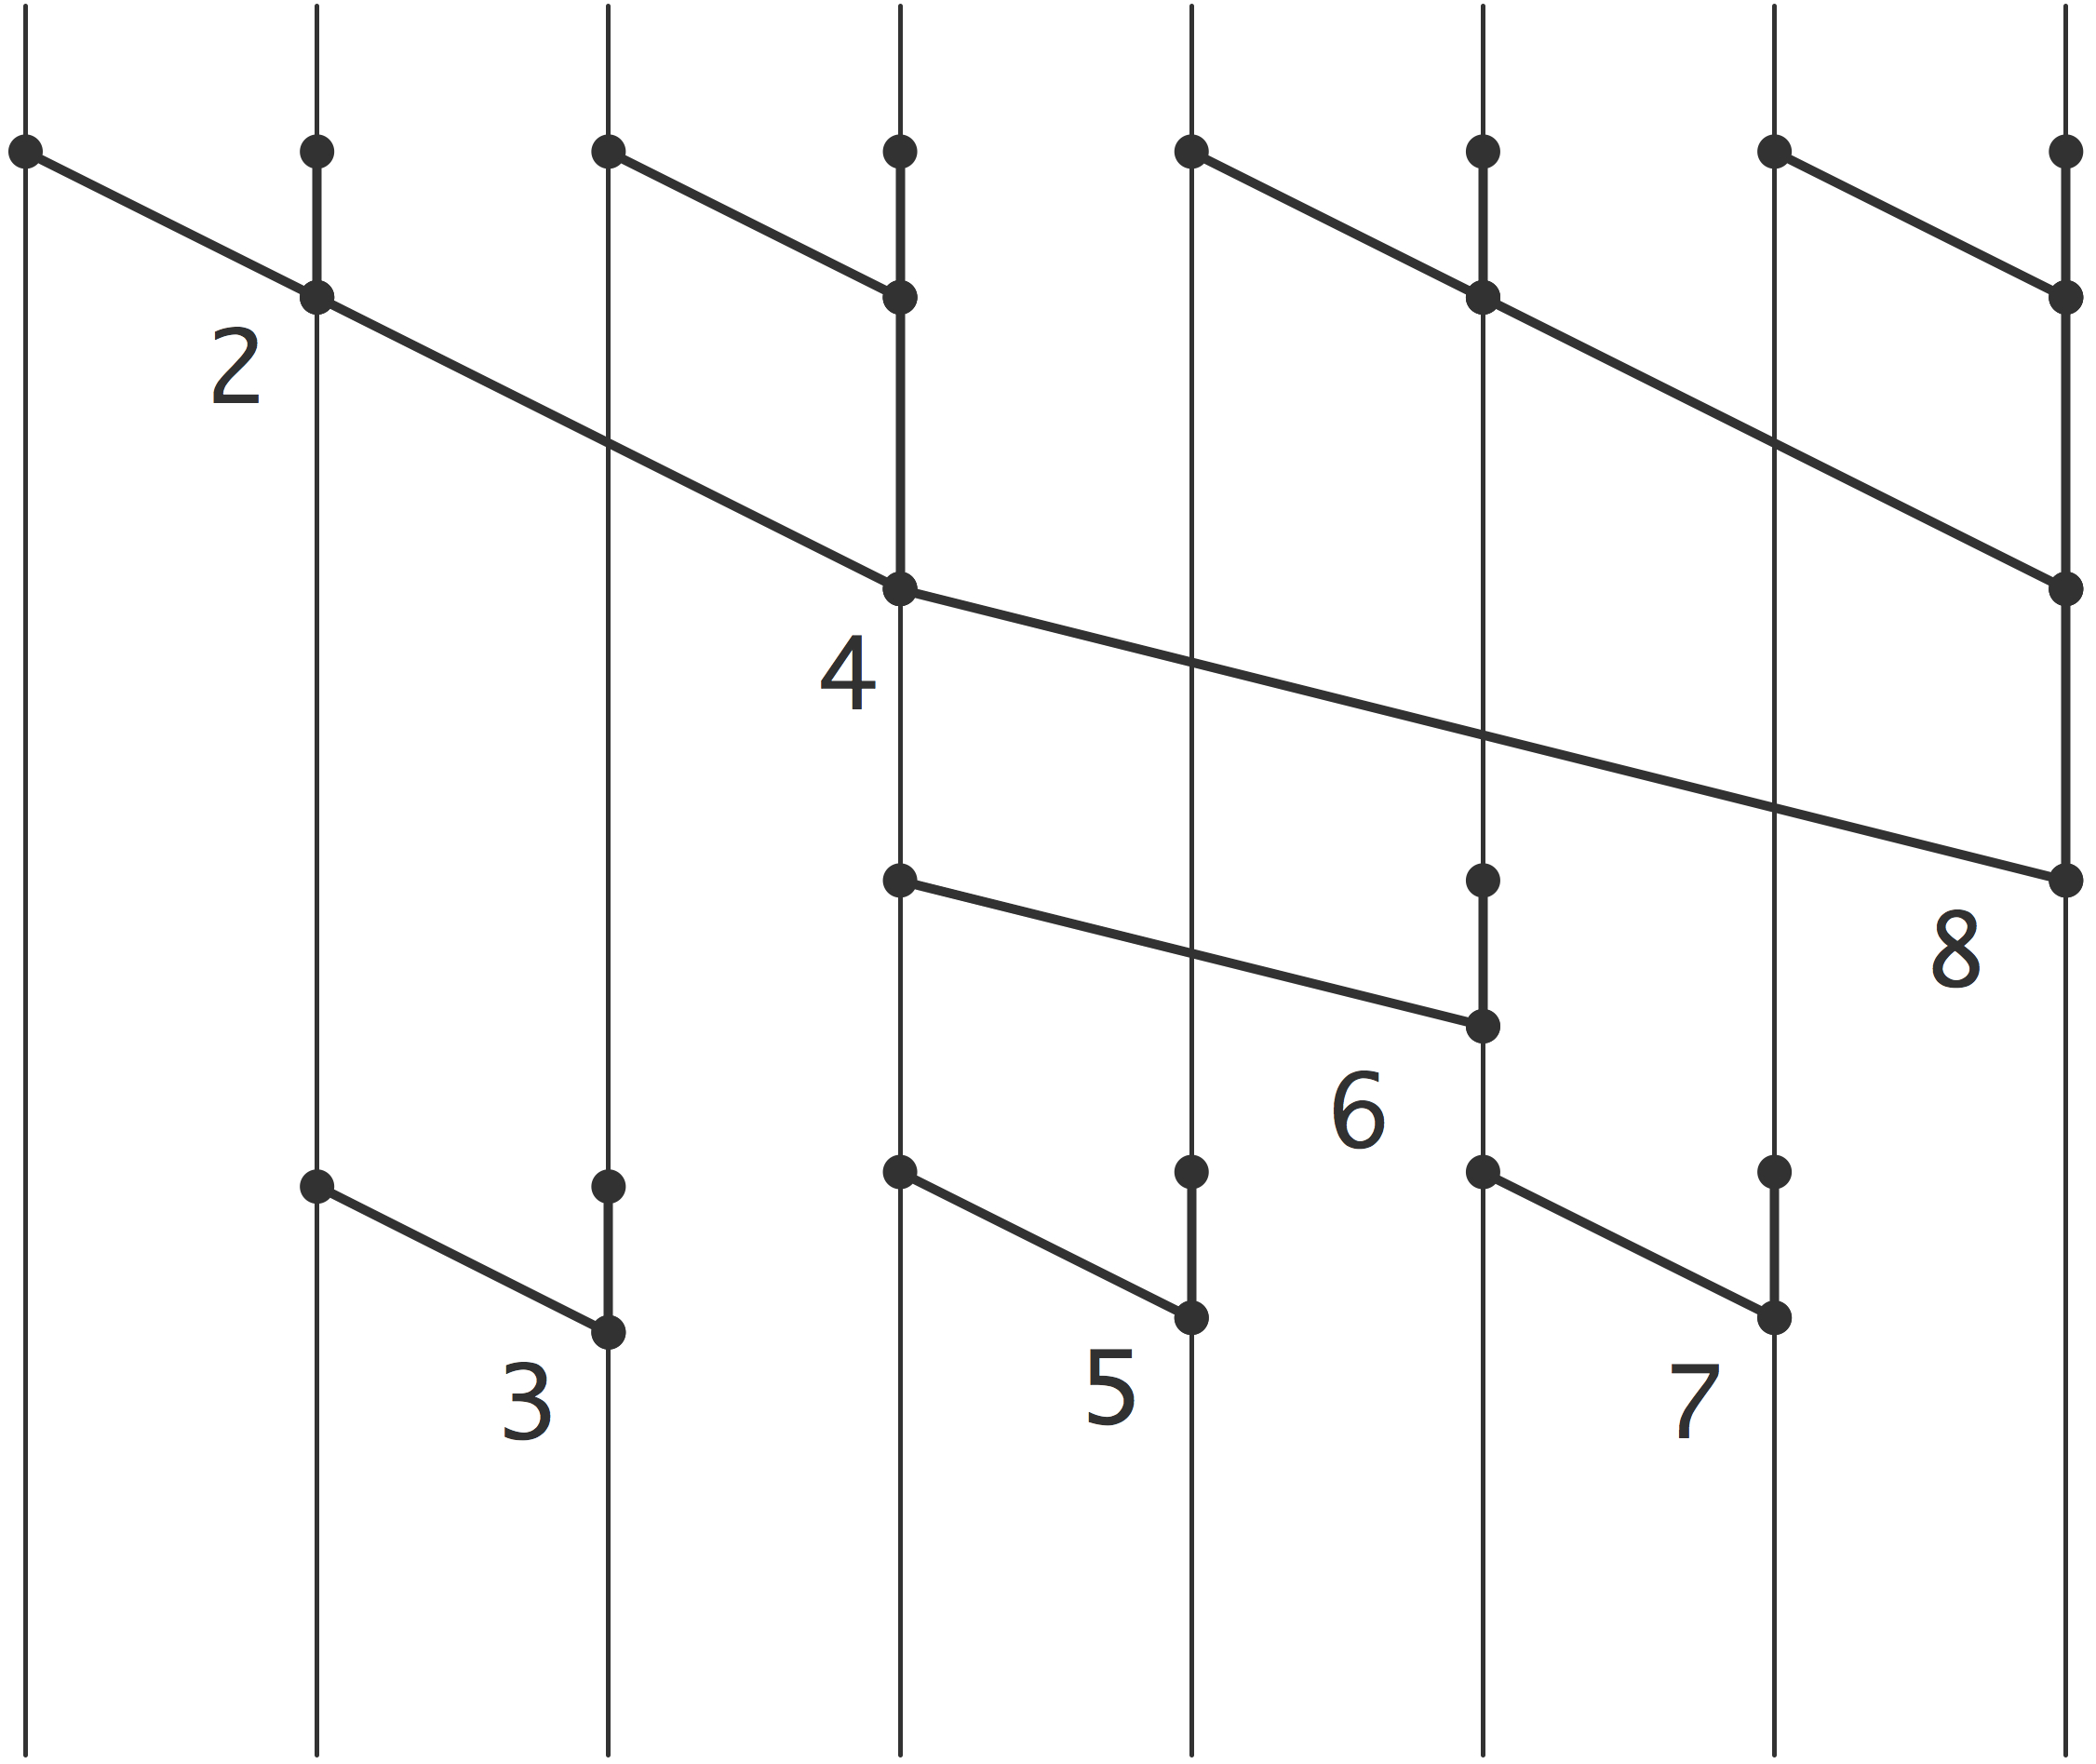
\includegraphics[scale=.1]{parallel-prefix}
  \caption{A prefix operation applied to 8 elements}
  \label{fig:prefix}
\end{figure}
To compute, say, $X_{13}$, you express $13=8+4+1$ and compute
$X_{13}=X_8\oplus X_{9,12} \oplus x_13$.

In this figure, operations over the same `distance' have been
horizontally aligned corresponding to a \ac{SIMD} type execution.
If the execution proceeds with a task graph, some steps can be
executed earlier than the figure suggests; for instance $X_3$ can be
computed simultaneously with~$X_6$.

Regardless the arrangement of the computational steps,
it is not hard to see that the whole prefix calculation
can be done in $2\log_2n$ steps: $\log_2 n$~steps for 
computing the final reduction~$X_n$, then another $\log_2 n$
steps for filling in the intermediate values.

\Level 1 {Sparse matrix vector product as parallel prefix}
\label{sec:spmvp-prefix}
\index{sparse!matrix-vector product!as parallel prefix|see{prefix operations!sparse matrix vector product}}
\index{prefix operations!sparse matrix vector product|(}

It has been observed that the sparse matrix vector product can be considered a prefix operation; 
see~\cite{Blelloc:segmented-report}.
The reasoning here is we first compute all $y_{ij}\equiv a_{ij}x_j$, and subsequently
compute the sums $y_i=\sum_j y_{ij}$ with a prefix operation.

A~prefix sum as explained above does not compute the right result. The first couple of $y_{ij}$ terms
do indeed sum to~$y_1$, but then continuing the prefix sum gives $y_1+y_2$, instead of~$y_2$.
The trick to making this work is to consider two-component quantities $\langle y_{ij},s_{ij}\rangle$,
where
\[ s_{ij} =
\begin{cases}
1&\hbox{if $j$ is the first nonzero index in row $i$}\\ 0&\hbox{otherwise}
\end{cases}
\]
Now we can define prefix sums that are `reset' every time $s_{ij}=1$.

\index{prefix operations!sparse matrix vector product|)}
